\documentclass[tikz,border=8pt]{standalone}
\usepackage{amsmath,amssymb}
\usetikzlibrary{arrows.meta,positioning,calc,fit,backgrounds,decorations.pathreplacing,shapes.geometric}
\begin{document}
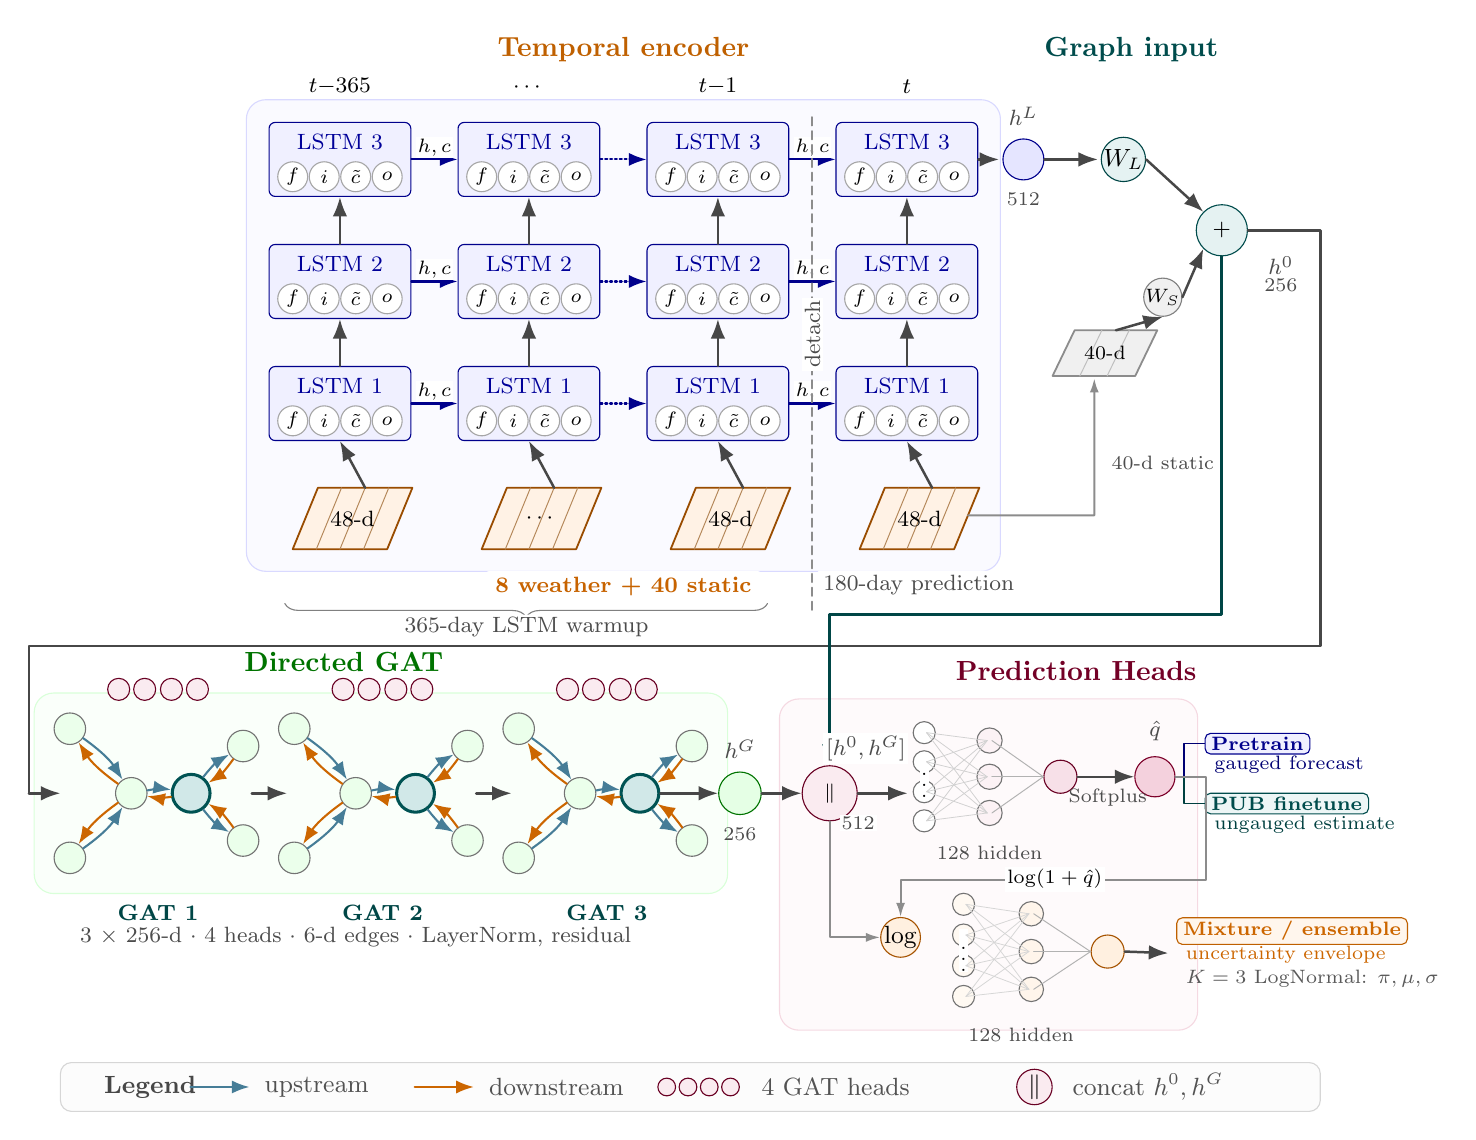
\begin{tikzpicture}[
  >=Latex,
  font=\rmfamily\small,
  line cap=round,
  line join=round,
  flow/.style={-Latex, line width=0.9pt, draw=black!72},
  softflow/.style={-{Latex[length=1.8mm,width=1.15mm]}, line width=0.75pt, draw=black!45},
  recur/.style={-Latex, line width=0.75pt, draw=blue!55!black},
  upedge/.style={-Latex, line width=0.75pt, draw=cyan!55!black},
  downedge/.style={-Latex, line width=0.75pt, draw=orange!80!black},
  skip/.style={-Latex, line width=1.0pt, draw=teal!55!black},
  note/.style={font=\footnotesize, text=black!70, align=center},
  tinylabel/.style={font=\scriptsize, text=black!70, align=center},
  gate/.style={circle, draw=black!35, fill=white, minimum size=3.8mm, inner sep=0pt, font=\scriptsize},
  neuron/.style={circle, draw=black!55, fill=white, minimum size=3.6mm, inner sep=0pt},
  graphnode/.style={circle, draw=black!55, fill=green!8, minimum size=4.0mm, inner sep=0pt},
  targetnode/.style={circle, draw=teal!65!black, line width=1.1pt, fill=teal!18, minimum size=4.8mm, inner sep=0pt},
  prebadge/.style={rounded corners=2pt,draw=blue!55!black,fill=blue!6,inner xsep=3pt,inner ysep=2pt,font=\scriptsize\bfseries,align=center,text=blue!55!black},
  finebadge/.style={rounded corners=2pt,draw=teal!60!black,fill=teal!7,inner xsep=3pt,inner ysep=2pt,font=\scriptsize\bfseries,align=center,text=teal!60!black},
  mixbadge/.style={rounded corners=2pt,draw=orange!75!black,fill=orange!7,inner xsep=3pt,inner ysep=2pt,font=\scriptsize\bfseries,align=center,text=orange!80!black}
]

% ---------- helpers ----------
\newcommand{\plate}[6]{%
  \coordinate (#1-sw) at (#2,#3);
  \coordinate (#1-se) at ($(#1-sw)+(#4,0)$);
  \coordinate (#1-ne) at ($(#1-se)+(0.32,#5)$);
  \coordinate (#1-nw) at ($(#1-sw)+(0.32,#5)$);
  \draw[fill=orange!10,draw=orange!60!black,line width=.65pt]
    (#1-sw)--(#1-se)--(#1-ne)--(#1-nw)--cycle;
  \draw[orange!55!black!65, line width=.35pt]
    ($(#1-sw)!0.25!(#1-se)$)--($(#1-nw)!0.25!(#1-ne)$)
    ($(#1-sw)!0.50!(#1-se)$)--($(#1-nw)!0.50!(#1-ne)$)
    ($(#1-sw)!0.75!(#1-se)$)--($(#1-nw)!0.75!(#1-ne)$);
  \node[font=\footnotesize,align=center] at ($(#1-sw)!0.5!(#1-ne)$) {#6};
}

\newcommand{\staticplate}[6]{%
  \coordinate (#1-sw) at (#2,#3);
  \coordinate (#1-se) at ($(#1-sw)+(#4,0)$);
  \coordinate (#1-ne) at ($(#1-se)+(0.28,#5)$);
  \coordinate (#1-nw) at ($(#1-sw)+(0.28,#5)$);
  \draw[fill=gray!12,draw=black!45,line width=.65pt]
    (#1-sw)--(#1-se)--(#1-ne)--(#1-nw)--cycle;
  \draw[black!25, line width=.35pt]
    ($(#1-sw)!0.33!(#1-se)$)--($(#1-nw)!0.33!(#1-ne)$)
    ($(#1-sw)!0.66!(#1-se)$)--($(#1-nw)!0.66!(#1-ne)$);
  \node[font=\scriptsize,align=center] at ($(#1-sw)!0.5!(#1-ne)$) {#6};
}

\newcommand{\lstmcell}[4]{%
  \node[rounded corners=2.2pt, draw=blue!55!black, fill=blue!6,
        minimum width=1.80cm, minimum height=.94cm, inner sep=1.5pt] (#1) at (#2,#3) {};
  \node[font=\footnotesize, text=blue!60!black] at ($(#1.center)+(0,.22)$) {#4};
  \node[gate] (#1-f) at ($(#1.center)+(-.60,-.22)$) {$f$};
  \node[gate] (#1-i) at ($(#1.center)+(-.20,-.22)$) {$i$};
  \node[gate] (#1-g) at ($(#1.center)+(.20,-.22)$) {$\tilde c$};
  \node[gate] (#1-o) at ($(#1.center)+(.60,-.22)$) {$o$};
}

\newcommand{\rivergraph}[4]{%
  \coordinate (#1-c) at (#2,#3);
  \node[graphnode] (#1-a) at ($(#1-c)+(-.78,.82)$) {};
  \node[graphnode] (#1-b) at ($(#1-c)+(-.78,-.82)$) {};
  \node[graphnode] (#1-d) at ($(#1-c)+(0,0)$) {};
  \node[targetnode] (#1-e) at ($(#1-c)+(.76,0)$) {};
  \node[graphnode] (#1-f) at ($(#1-c)+(1.42,.60)$) {};
  \node[graphnode] (#1-g) at ($(#1-c)+(1.42,-.60)$) {};
  \draw[upedge,bend left=11] (#1-a) to (#1-d);
  \draw[downedge,bend left=11] (#1-d) to (#1-a);
  \draw[upedge,bend right=11] (#1-b) to (#1-d);
  \draw[downedge,bend right=11] (#1-d) to (#1-b);
  \draw[upedge,bend left=10] (#1-d) to (#1-e);
  \draw[downedge,bend left=10] (#1-e) to (#1-d);
  \draw[upedge,bend left=11] (#1-e) to (#1-f);
  \draw[downedge,bend left=11] (#1-f) to (#1-e);
  \draw[upedge,bend right=11] (#1-e) to (#1-g);
  \draw[downedge,bend right=11] (#1-g) to (#1-e);
  \foreach \dx in {-0.50,-0.17,0.17,0.50}{
     \node[circle,draw=purple!55!black,fill=purple!8,minimum size=2.8mm,inner sep=0pt]
       at ($(#1-c)+(0.34+\dx,1.32)$) {};
  }
  \node[font=\footnotesize\bfseries,align=center,text=teal!55!black]
    at ($(#1-c)+(0.34,-1.52)$) {GAT #4};
}

% Output projection, Softplus activation, directed edge legend, and GAT layers
% by replacing existing labels, not by adding new panels.
% Caption carries the title.

% ================================================================
% ROW 1: temporal encoder + graph-input projection
% ================================================================
\node[font=\normalsize\bfseries,text=orange!75!black] at (8.70,11.70) {Temporal encoder};

% Four representative time columns (restore the explicit omitted-time column)
\foreach \x/\tag in {5.10/$t{-}365$,7.50/$\cdots$,9.90/$t{-}1$,12.30/$t$}{
  \node[font=\footnotesize\bfseries] at (\x,11.22) {\tag};
}

% Input plates
\plate{inA}{4.50}{5.35}{1.20}{.78}{48-d}
\plate{inB}{6.90}{5.35}{1.20}{.78}{$\cdots$}
\plate{inC}{9.30}{5.35}{1.20}{.78}{48-d}
\plate{inD}{11.70}{5.35}{1.20}{.78}{48-d}
\node[font=\footnotesize\bfseries,text=orange!78!black,fill=white,rounded corners=1.5pt,
      inner xsep=4pt,inner ysep=2pt] at (8.70,4.88) {8 weather + 40 static};

% LSTM stacks
\foreach \x/\pfx in {5.10/A,7.50/B,9.90/C,12.30/D}{
  \lstmcell{\pfx-one}{\x}{7.20}{LSTM 1}
  \lstmcell{\pfx-two}{\x}{8.75}{LSTM 2}
  \lstmcell{\pfx-three}{\x}{10.30}{LSTM 3}
  \draw[flow] (\pfx-one.north) -- (\pfx-two.south);
  \draw[flow] (\pfx-two.north) -- (\pfx-three.south);
}
\draw[flow] ($(inA-nw)!0.5!(inA-ne)$) -- (A-one.south);
\draw[flow] ($(inB-nw)!0.5!(inB-ne)$) -- (B-one.south);
\draw[flow] ($(inC-nw)!0.5!(inC-ne)$) -- (C-one.south);
\draw[flow] ($(inD-nw)!0.5!(inD-ne)$) -- (D-one.south);

% Recurrent h,c connections
\foreach \aa/\bb in {A-one/B-one,A-two/B-two,A-three/B-three}{
  \draw[recur] (\aa.east) -- node[above,font=\scriptsize,fill=white,inner sep=.7pt] {$h,c$} (\bb.west);
}
\foreach \aa/\bb in {B-one/C-one,B-two/C-two,B-three/C-three}{
  \draw[recur,densely dotted] (\aa.east) -- (\bb.west);
}
\foreach \aa/\bb in {C-one/D-one,C-two/D-two,C-three/D-three}{
  \draw[recur] (\aa.east) -- node[above,font=\scriptsize,fill=white,inner sep=.7pt] {$h,c$} (\bb.west);
}

% Warmup / detach / prediction labels
\draw[decorate,decoration={brace,mirror,amplitude=5pt},draw=black!50]
  (4.40,4.66) -- (10.53,4.66);
\node[note,fill=white,rounded corners=1pt,inner xsep=2pt,inner ysep=1pt]
  at (7.47,4.36) {365-day LSTM warmup};
\draw[densely dashed,black!45,line width=.7pt] (11.10,4.58) -- (11.10,10.84);
\node[note,rotate=90,fill=white,inner sep=1pt] at (11.10,8.08) {detach};
\node[note,align=center,fill=white,rounded corners=1pt,inner xsep=2.2pt,inner ysep=1.5pt] at (12.45,4.90) {180-day prediction};

% hL and graph input on the same row, so the top row fills naturally
\node[neuron,fill=blue!10,draw=blue!55!black,minimum size=5.2mm] (hL) at (13.78,10.30) {};
\draw[flow,shorten >=1.2pt] (D-three.east) -- (hL.west);
\node[note,above=1pt of hL] {$h^L$};
\node[tinylabel,below=1pt of hL] {512};

\node[font=\normalsize\bfseries,text=teal!60!black] at (15.15,11.70) {Graph input};
\node[neuron,fill=teal!10,draw=teal!55!black,minimum size=5mm] (WL) at (15.05,10.30) {$W_L$};
\node[neuron,fill=teal!10,draw=teal!60!black,minimum size=6.5mm,font=\footnotesize] (sum) at (16.30,9.40) {$+$};
\draw[flow,shorten >=1.0pt] (hL.east) -- (WL.west);
\draw[flow] (WL.east) -- (sum.north west);
% Branch the static part of the 48-d input (not the weather) into W_S.
\staticplate{stat}{14.15}{7.55}{1.05}{0.58}{40-d}
\draw[softflow] ($(inD-se)!0.55!(inD-ne)$) -- (14.68,5.78) -- (14.68,7.52);
\node[tinylabel,fill=white,inner sep=1pt,align=center] at (15.55,6.45) {40-d static};
\node[neuron,fill=gray!12,draw=black!50,minimum size=4.6mm,font=\scriptsize] (WS) at (15.55,8.55) {$W_S$};
\draw[flow] ($(stat-nw)!0.5!(stat-ne)$) -- (WS.south);
\draw[flow] (WS.east) -- (sum.south west);
\node[note,fill=white,inner sep=1pt] at (17.05,8.95) {$h^0$};
\node[tinylabel,fill=white,inner sep=.7pt] at (17.05,8.70) {256};

% Row transition: routed only through the gap between rows.
\draw[line width=0.9pt,draw=black!72] (sum.east) -- (17.55,9.40) -- (17.55,4.12) -- (1.15,4.12) -- (1.15,2.25);

% ================================================================
% ROW 2: Directed GAT + concat + Prediction Heads
% ================================================================
\node[font=\normalsize\bfseries,text=green!45!black] at (5.15,3.92) {Directed GAT};

\rivergraph{G1}{2.45}{2.25}{1}
\rivergraph{G2}{5.30}{2.25}{2}
\rivergraph{G3}{8.15}{2.25}{3}

% connect row-turn into first graph and between graph stages
% Deliberately leave visible shaft length before each arrowhead.
\draw[flow] (1.15,2.25) -- (1.55,2.25);
\draw[flow] (3.98,2.25) -- (4.43,2.25);
\draw[flow] (6.83,2.25) -- (7.28,2.25);

\node[note,align=center] at (5.30,.42)
  {3 $\times$ 256-d $\cdot$ 4 heads $\cdot$ 6-d edges $\cdot$ LayerNorm, residual};

% final graph state
\node[neuron,fill=green!10,draw=green!45!black,minimum size=5.4mm] (hG) at (10.18,2.25) {};
\draw[flow] (G3-e.east) -- (hG.west);
\node[note,above=1pt of hG] {$h^G$};
\node[tinylabel,below=1pt of hG] {256};

% concatenate hG with h0; route h0 along bottom edge using straight segments
\node[neuron,fill=purple!8,draw=purple!55!black,minimum size=7mm,font=\scriptsize] (concat) at (11.32,2.25) {$\Vert$};
\draw[flow] (hG.east) -- (concat.west);
\draw[skip] (sum.south) -- (16.30,4.52) -- (11.32,4.52) -- (11.32,2.65) -- (concat.north);
\node[note,fill=white,inner sep=1pt] at (11.78,2.82) {$[h^0,h^G]$};
\node[tinylabel,fill=white,inner sep=.7pt] at (11.68,1.87) {512};

% Prediction heads occupy the right half of row 2
\node[font=\normalsize\bfseries,text=purple!60!black] at (14.45,3.80) {Prediction Heads};

% Point head - a few representative neurons keep the MLP readable
\node[neuron,minimum size=2.8mm] (ptop) at (12.52,3.02) {};
\foreach \yy in {2.65,2.27,1.90}{
  \node[neuron,minimum size=2.8mm] at (12.52,\yy) {};
}
\node at (12.52,2.46) [font=\scriptsize,fill=white,inner sep=.45pt] {$\vdots$};
\foreach \yy in {2.92,2.46,2.00}{
  \node[neuron,minimum size=3.2mm,fill=purple!5] at (13.35,\yy) {};
}
\node (qraw) [neuron,minimum size=4.2mm,fill=purple!12,draw=purple!55!black] at (14.25,2.46) {};
\draw[flow] (concat.east) -- (12.31,2.25);
\foreach \ya in {1.90,2.27,2.65,3.02}{
  \foreach \yb in {2.00,2.46,2.92}{
    \draw[black!18,line width=.28pt] (12.55,\ya) -- (13.32,\yb);
  }
}
\foreach \yb in {2.00,2.46,2.92}{
  \draw[black!30,line width=.35pt] (13.38,\yb) -- (qraw.west);
}
\node[tinylabel] at (13.35,1.50) {128 hidden};
\node[neuron,minimum size=5.1mm,fill=purple!18,draw=purple!65!black] (qhat) at (15.45,2.46) {};
\draw[flow] (qraw.east) -- (qhat.west);
\node[note,above=2pt of qhat] {$\hat q$};
\node[tinylabel] at (14.85,2.20) {Softplus};
% Compact stage labels: short tags keep the output area uncluttered.
\draw[blue!45!black,line width=.55pt] (qhat.east) -- (15.82,2.46) -- (15.82,2.88) -- (16.08,2.88);
\node[prebadge,anchor=west,inner xsep=2.3pt,inner ysep=1.3pt] at (16.08,2.88) {Pretrain};
\node[font=\scriptsize,text=blue!45!black,anchor=west] at (16.08,2.61) {gauged forecast};
\draw[teal!50!black,line width=.55pt] (qhat.east) -- (15.82,2.46) -- (15.82,2.12) -- (16.08,2.12);
\node[finebadge,anchor=west,inner xsep=2.3pt,inner ysep=1.3pt] at (16.08,2.12) {PUB finetune};
\node[font=\scriptsize,text=teal!50!black,anchor=west] at (16.08,1.85) {ungauged estimate};

% MDN head, compactly placed beneath point head but still within row 2 footprint
\node[neuron,minimum size=4.5mm,fill=orange!12,draw=orange!65!black] (logq) at (12.22,.42) {$\log$};
\draw[softflow] (qhat.east) -- (16.10,2.46) -- (16.10,1.15) -- (12.22,1.15) -- (logq.north);
\node[font=\scriptsize,fill=white,inner sep=1pt] at (14.18,1.16) {$\log(1+\hat q)$};
\draw[softflow] (concat.south) |- (logq.west);

\foreach \yy in {.84,.45,.06}{
  \node[neuron,minimum size=2.8mm,fill=orange!5] at (13.02,\yy) {};
}
\node[neuron,minimum size=2.8mm,fill=orange!5] (pbot) at (13.02,-.33) {};
\node at (13.02,.25) [font=\scriptsize,fill=white,inner sep=.4pt] {$\vdots$};
\foreach \yy in {.72,.24,-.24}{
  \node[neuron,minimum size=3.1mm,fill=orange!8] at (13.88,\yy) {};
}
\foreach \ya in {-.33,.06,.45,.84}{
  \foreach \yb in {-.24,.24,.72}{
    \draw[black!16,line width=.28pt] (13.05,\ya) -- (13.85,\yb);
  }
}
\node[tinylabel,align=center] at (13.75,-.82) {128 hidden};
\node[neuron,minimum size=4.2mm,fill=orange!12,draw=orange!65!black] (mdnout) at (14.85,.24) {};
\foreach \yb in {-.24,.24,.72}{
  \draw[black!30,line width=.35pt] (13.91,\yb) -- (mdnout.west);
}
\draw[flow] (mdnout.east) -- (15.62,.22);
\node[mixbadge,anchor=west,inner xsep=2.3pt,inner ysep=1.3pt] at (15.72,.50) {Mixture / ensemble};
\node[font=\scriptsize,text=orange!80!black,anchor=west] at (15.72,.20) {uncertainty envelope};
\node[font=\scriptsize,text=black!65,anchor=west] at (15.72,-.10) {$K=3$ LogNormal: $\pi,\mu,\sigma$};


% ---------- compact legend ----------
\node[font=\small\bfseries,text=black!72,anchor=west] at (1.98,-1.48) {Legend};

% Replace the single blue link with the two directed colors already on the graph.
\draw[upedge] (3.20,-1.48) -- (3.95,-1.48);
\node[font=\small,anchor=west,text=black!68] at (4.02,-1.48) {upstream};
\draw[downedge] (6.05,-1.48) -- (6.80,-1.48);
\node[font=\small,anchor=west,text=black!68] at (6.87,-1.48) {downstream};

% Four GAT attention heads
\foreach \xx in {9.25,9.52,9.79,10.06}{
  \node[circle,draw=purple!55!black,fill=purple!8,minimum size=2.25mm,inner sep=0pt] at (\xx,-1.48) {};
}
\node[font=\small,anchor=west,text=black!68] at (10.33,-1.48) {4 GAT heads};

% Concatenation symbol
\node[neuron,fill=purple!8,draw=purple!55!black,minimum size=4.5mm,font=\small] (legcat) at (13.92,-1.48) {$\Vert$};
\node[font=\small,anchor=west,text=black!68] at (14.28,-1.48) {concat $h^0,h^G$};

\begin{scope}[on background layer]
  \node[rounded corners=4pt,fill=black!1,draw=black!16,
        minimum width=16.0cm,minimum height=.62cm] at (9.55,-1.48) {};
\end{scope}

% ---------- subtle group backgrounds ----------
\begin{scope}[on background layer]
  \node[rounded corners=7pt,fill=blue!2,draw=blue!15,
        fit=(A-one)(D-three)(inA-ne)(inD-sw),inner sep=8pt] {};
  \node[rounded corners=7pt,fill=green!2,draw=green!15,
        fit=(G1-a)(G3-f)(G1-b)(G3-g),inner sep=7pt] {};
  \node[rounded corners=7pt,fill=purple!2,draw=purple!15,
        fit=(concat)(qhat)(logq)(mdnout)(ptop)(pbot),inner sep=8pt] {};
\end{scope}

\end{tikzpicture}
\end{document}
